\cleardoublepage

\section{预备知识}
在本节,我们将给出一些符号和定义。在之后的部分,我们会直接使用这些符号和结论。
\subsection{基础符号}
首先定义计算域$[a,b]$的一个剖分
\begin{align*}
    I_{j} = (x_{j-1/2}, x_{j+1/2}), \ j = 1, 2, ..., N
\end{align*}
其中$a=x_{1/2} < x_{3/2}< ...< x_{N+1/2}=b$,N表示网格数。接着定义
\begin{align*}
    \Delta x_j = x_{j+1/2}-x_{j-1/2}, \quad h = \max{\sup_j{\Delta x_j}}, \quad x_j = (x_{j+1/2}+x_{j-1/2})/{2},
\end{align*}
其中$\Delta x_j$表示网格大小,$h$表示网格长度,$x_j$表示网格中点。

网格上有限维计算空间$V_h^k = \{v:v|_{I_j}\in P^k(I_j); 1\leq j\leq N\}$,其中$P^k(I_j)$表示$I_j$上次数不大于$k$的多项式集合。我们的数值解和测试函数都将从$V_h^k$中取得。需要注意的是,$V_h^k$中的函数在单元边界节点处不一定是连续的,可以出现跳跃。

为了简化标记,我们分别定义$(u_h)^+_{j+1/2}=u_h(x^+_{j+1/2})$和$(u_h)^-_{j+1/2}=u_h(x^-_{j+1/2})$。此外我们定义$u_h$在单元边界节点$x_{j+1/2}$的跳跃$[u_h]_{j+1/2}=(u_h)^+_{j+1/2}-(u_h)^-_{j+1/2}$和均值$(\overline{u}_h)_{j+1/2}=((u_h)_{j+1/2}^++(u_h)_{j+1/2}^-)/2$。
\subsection{初值的处理}
我们的初值函数就是定义在$[0, 0.6]$的掺杂函数$n_d$,它满足
\begin{align*}
    n_d(x) = \begin{cases}
                 5\times 10^{17}, \quad x \in [0, 0.1] \cup [0.5, 0.6] \\
                 2\times 10^{15}, \quad x \in [0.15,0.45]
             \end{cases}
\end{align*}
在中间过渡区域选择光滑的函数连接。在本文中我们考虑光滑过渡函数$g(x)$,满足
\begin{align*}
    f(x)               & ={\begin{cases}
                               e^{-{\frac {1}{x}}}, \quad x>0 \\
                               0, \quad x\leq 0\end{cases}} ,                     \\
    \displaystyle g(x) & :={\frac {f(x)}{f(x)+f(1-x)}}\quad x\in \mathbb {R}.
\end{align*}
为了得到区间$[a,b]$上的光滑过渡,我们只需要考虑函数
\begin{align*}
    g(\frac{x-a}{b-a}).
\end{align*}
注意到它任意阶导函数在$[a,b]$外都为零,结合掺杂函数我们容易得到一个任意阶连续导函数的初值函数。这不是唯一可选择的过渡函数,但由于初值函数的光滑性与计算空间的维数有关,选择这样一个绝对光滑的初值函数可以简化后续分析。

为了让初值函数落在我们的计算空间中,我们需要对其进行处理。本文选择的是向计算空间$V_h^k$的分段$L^2$投影,表示为$\mathcal{P}$。对于任意函数$u\in C^{k+1}$,它满足
\begin{align}
    \int_{I_j}(\mathcal{P}u(x)-u(x)v(x)) \rm{d}x = 0, \quad \forall v \in P^k(I_j).
\end{align}

\section{DD模型}
本文采用的DD模型表示为
\begin{align}
    n_t - (\mu En)_x = \tau \theta n_{xx}, \label{eq:DD} \\
    \phi_{xx} = \frac{e}{\epsilon}(n - n_d),  \label{eq:poisson},
\end{align}
其中$x\in(0,1)$,第一个电子浓度方程取周期边界条件,第二个电势方程取Dirichlet边界条件:$\phi(0,t) = 0, \phi(1,t) = v_{bias}$。
在系统\eqref{eq:DD}-\eqref{eq:poisson}中,未知量是电子浓度$n$和电势$\phi$。$m_0$表示电子有效质量,k是Boltzmann常数,e是电子电荷,$\mu$代表迁移率,$T_0$是晶格温度,$\tau = \frac{m_0 \mu}{e}$是松弛参数,$\theta = \frac{k}{m_0}T_0$,$\epsilon$是介电常量,$n_d$是一个给定的掺杂函数。

\subsection{弱形式和LDG格式}
我们有以下事实\cite{sullivan2020brief}:
\begin{itemize}
    \item 许多PDEs没有强解但有弱解
    \item 弱解更容易在线性代数表示
    \item 即使强解存在,证明弱解存在性再说明其具有强解的性质往往比直接找到一个强解要简单
\end{itemize}
而我们的DD模型的强解很难求出,因此我们期望弱化要求,求得一个对于测试函数满足我们真正关心的性质的弱解,这同时也能给我们带来编程上的简便。

为了得到这样的弱解,我们想法是在方程\eqref{eq:DD}-\eqref{eq:poisson}两边乘上测试函数并积分得到弱形式,利用数值方法求解弱形式。

而DGM的想法就是找到独一无二的数值解$n_h^k\in V_h^k$使得对于任意的测试函数,弱形式都成立。但是由于DG难以处理高阶问题,因此我们需要考虑局部间断伽辽金法(LDG)。LDG法的想法是引入一个辅助变量来使得含有高阶偏导的PDE降阶为只含一阶导的PDEs,进而可以在这些一阶PDEs上应用DG法。
取$q = \sqrt{\tau \theta }n_x$,那么\autoref{eq:DD}可以写作
\begin{align}
    n_t - (\mu E n)_x - \sqrt{\tau \theta}q_x & = 0, \label{eq:DD:electronConcentration} \\
    q - \sqrt{\tau \theta}n_x                 & = 0. \label{eq:DD:auxiliaryFunction}
\end{align}
而对于泊松方程,本文直接通过积分得到。

令$E = -\phi_x$表示电势,通过引入辅助变量易证$E$具有周期性\cite{liu2010errorc}。

在方程\eqref{eq:DD:electronConcentration}-\eqref{eq:DD:auxiliaryFunction}两边分别乘以测试函数$v,w\in V_h^k$,分部积分得到
\begin{align}
     & \int_{I_{j}} n_{t} v d x+\int_{I_{j}}(\mu E n+\sqrt{\tau \theta} q) v_{x} d x                                                                               \nonumber                     \\
     & \quad-(\mu E n+\sqrt{\tau \theta} q)_{j+\frac{1}{2}} v_{j+\frac{1}{2}}^{-}+(\mu E n+\sqrt{\tau \theta} q)_{j-\frac{1}{2}} v_{j-\frac{1}{2}}^{+}=0,                                        \\
     & \int_{I_{j}} q w d x+\int_{I_{j}} \sqrt{\tau \theta} n w_{x} d x-\sqrt{\tau \theta} n_{j+\frac{1}{2}} w_{j+\frac{1}{2}}^{-}+\sqrt{\tau \theta} n_{j-\frac{1}{2}} w_{j-\frac{1}{2}}^{+}=0, \\
     & E_{x}=-\frac{e}{\varepsilon}\left(n-n_{d}\right) .
\end{align}
将上述方程中的精确解$n, q$和$E$替换为它们在$V_{h}^{k}$中的数值近似解$n^{h}, q^{h}$。由于数值解$n^{h}$和$q^{h}$在单元边界上不连续性,将单元边界上的项替换为适当的数值通量,我们得到LDG格式:
\begin{align}
     & \int_{I_{j}}\left(n^{h}\right)_{t} v d x+\int_{I_{j}}\left(\mu E^{h} n^{h}+\sqrt{\tau \theta} q^{h}\right) v_{x} d x      \nonumber                                                                                                                \\
     & \quad-\left(\mu \widehat{E^{h} n^{h}}+\sqrt{\tau \theta} \hat{q}^{h}\right)_{j+\frac{1}{2}} v_{j+\frac{1}{2}}^{-}+\left(\mu \widehat{E^{h} n^{h}}+\sqrt{\tau \theta} \hat{q}^{h}\right)_{j-\frac{1}{2}} v_{j-\frac{1}{2}}^{+}=0, \label{eq:DDLDGn} \\
     & \int_{I_{j}} q^{h} w d x+\int_{I_{j}} \sqrt{\tau \theta} n^{h} w_{x} d x-\sqrt{\tau \theta} \hat{n}_{j+\frac{1}{2}}^{h} w_{j+\frac{1}{2}}^{-}+\sqrt{\tau \theta} \hat{n}_{j-\frac{1}{2}}^{h} w_{j-\frac{1}{2}}^{+}=0,            \label{eq:DDLDGq} \\
     & E^{h}=\int_{0}^{x}-\frac{e}{\varepsilon}\left(n^{h}-n_{d}\right) d x+E_{0}-v_{\text {bias }},\label{eq:DDLDGE}
\end{align}
其中,$E_{0}=E^{h}(0)=\int_{0}^{1}\left(\int_{0}^{x} \frac{e}{\varepsilon}\left(n^{h}-n_{d}\right) d s\right) d x$。这里的“$\hat{}$”项表示数值通量。$\hat{n}^{h}$和$\hat{q}^{h}$选择交替通量,即$\hat{n}^{h}=\left(n^{h}\right)^{+}$,$\hat{q}^{h}=\left(q^{h}\right)^{-}$,$\widehat{E^{h} n^{h}}$采用上风通量,即$\widehat{E^{h} n^{h}}=\max \left(E^{h}, 0\right)\left(n^{h}\right)^{+}+\min \left(E^{h}, 0\right)\left(n^{h}\right)^{-}$。

从LDG格式可知,只要有m时间层的信息,我们可以仅从\eqref{eq:DDLDGq}求得辅助变量$q$,进而求得$m+1$时间层的数值解。这种只需要系统中一个方程求得辅助变量,因此我们这种方法为“局部”间断伽辽金法。这也是与过去需要全局系统才能求出$q$的方法的不同之处。

对于时间离散,我们采用三阶全变差不增(TVD)龙格库塔法。
\begin{align}
    u^{(1)} & = u^n + \Delta t L(u^n),                                                \\
    u^{(2)} & = \frac{3}{4}u^n + \frac{1}{4}u^{(1)} + \frac{1}{4}\Delta t L(u^{(1)}), \\
    u^{n+1} & = \frac{1}{3}u^n + \frac{2}{3}u^{(2)} + \frac{2}{3}\Delta t L(u^{(2)}).
\end{align}
该方法保证$TV(u^{n+1})\leq TV(u^n)$,其中$TV(u) = \sum_j |u_{j+1}-u_j|$。

\subsection{数值模拟}
我们取$T_0 = 300, k = 0.138 \times 10^{-4}, \epsilon = 11.7\times 8.85418, e = 0.1602, m = 0.26\times0.9109\times 10^{-31}, \mu = 0.75 $或$0.008(1+14.2273/(1+n_d/143200))$。边界条件$\phi=\phi_0=kT/e ln(n_d/n_i)$在左边界,$\phi = \phi_0+v_{bias}, v_{bias}=1.5$在右边界。在两个边界都有$T=300, n = 5\times 10^5$。

基函数选择放缩的正交归一化的勒让德多项式基,它的好处是质量矩阵恰好为单位阵,从而简化运算。初始函数$n_d$的图像如图
\begin{figure}
    \centering
    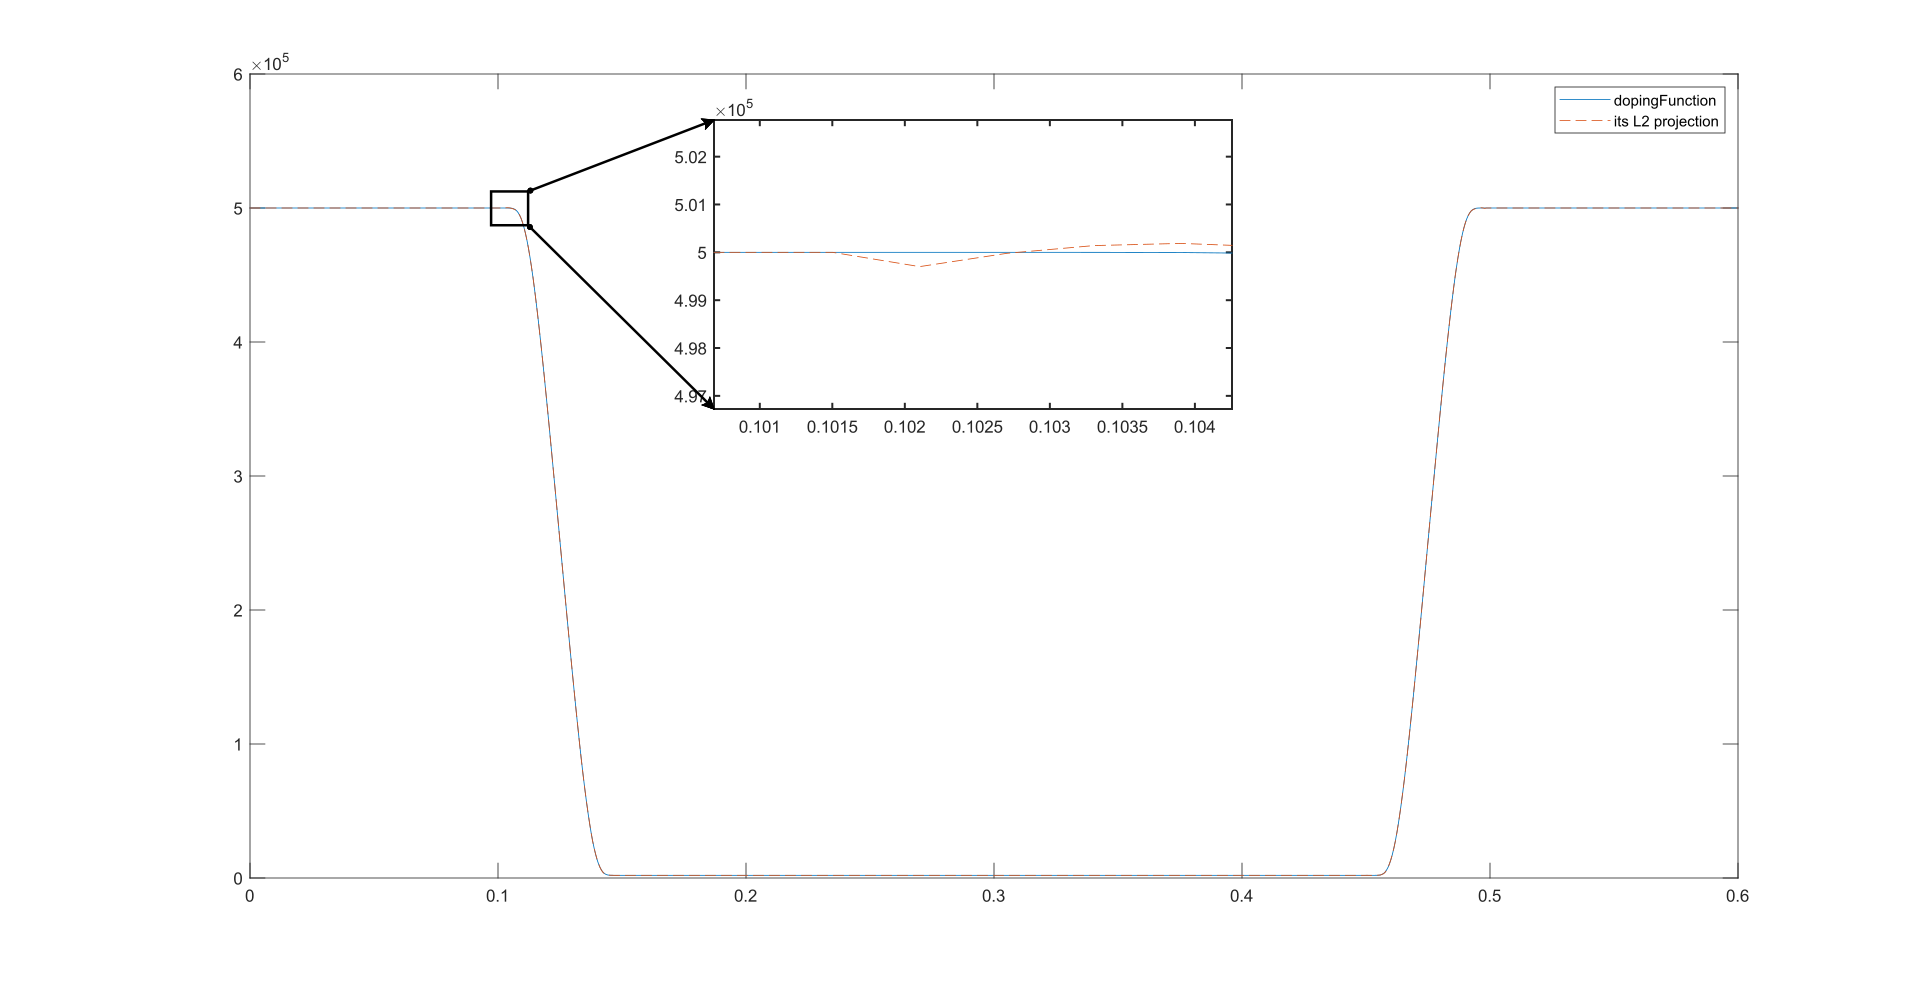
\includegraphics[width=\linewidth]{figure/dopingFunctionandL2projection.jpg}
    \caption{\small 100网格单元是掺杂函数以及它在$V_h^2$上的$L^2$投影}
\end{figure}

\begin{figure}
    \centering
    \begin{minipage}[b]{0.48\textwidth}
        \centering
        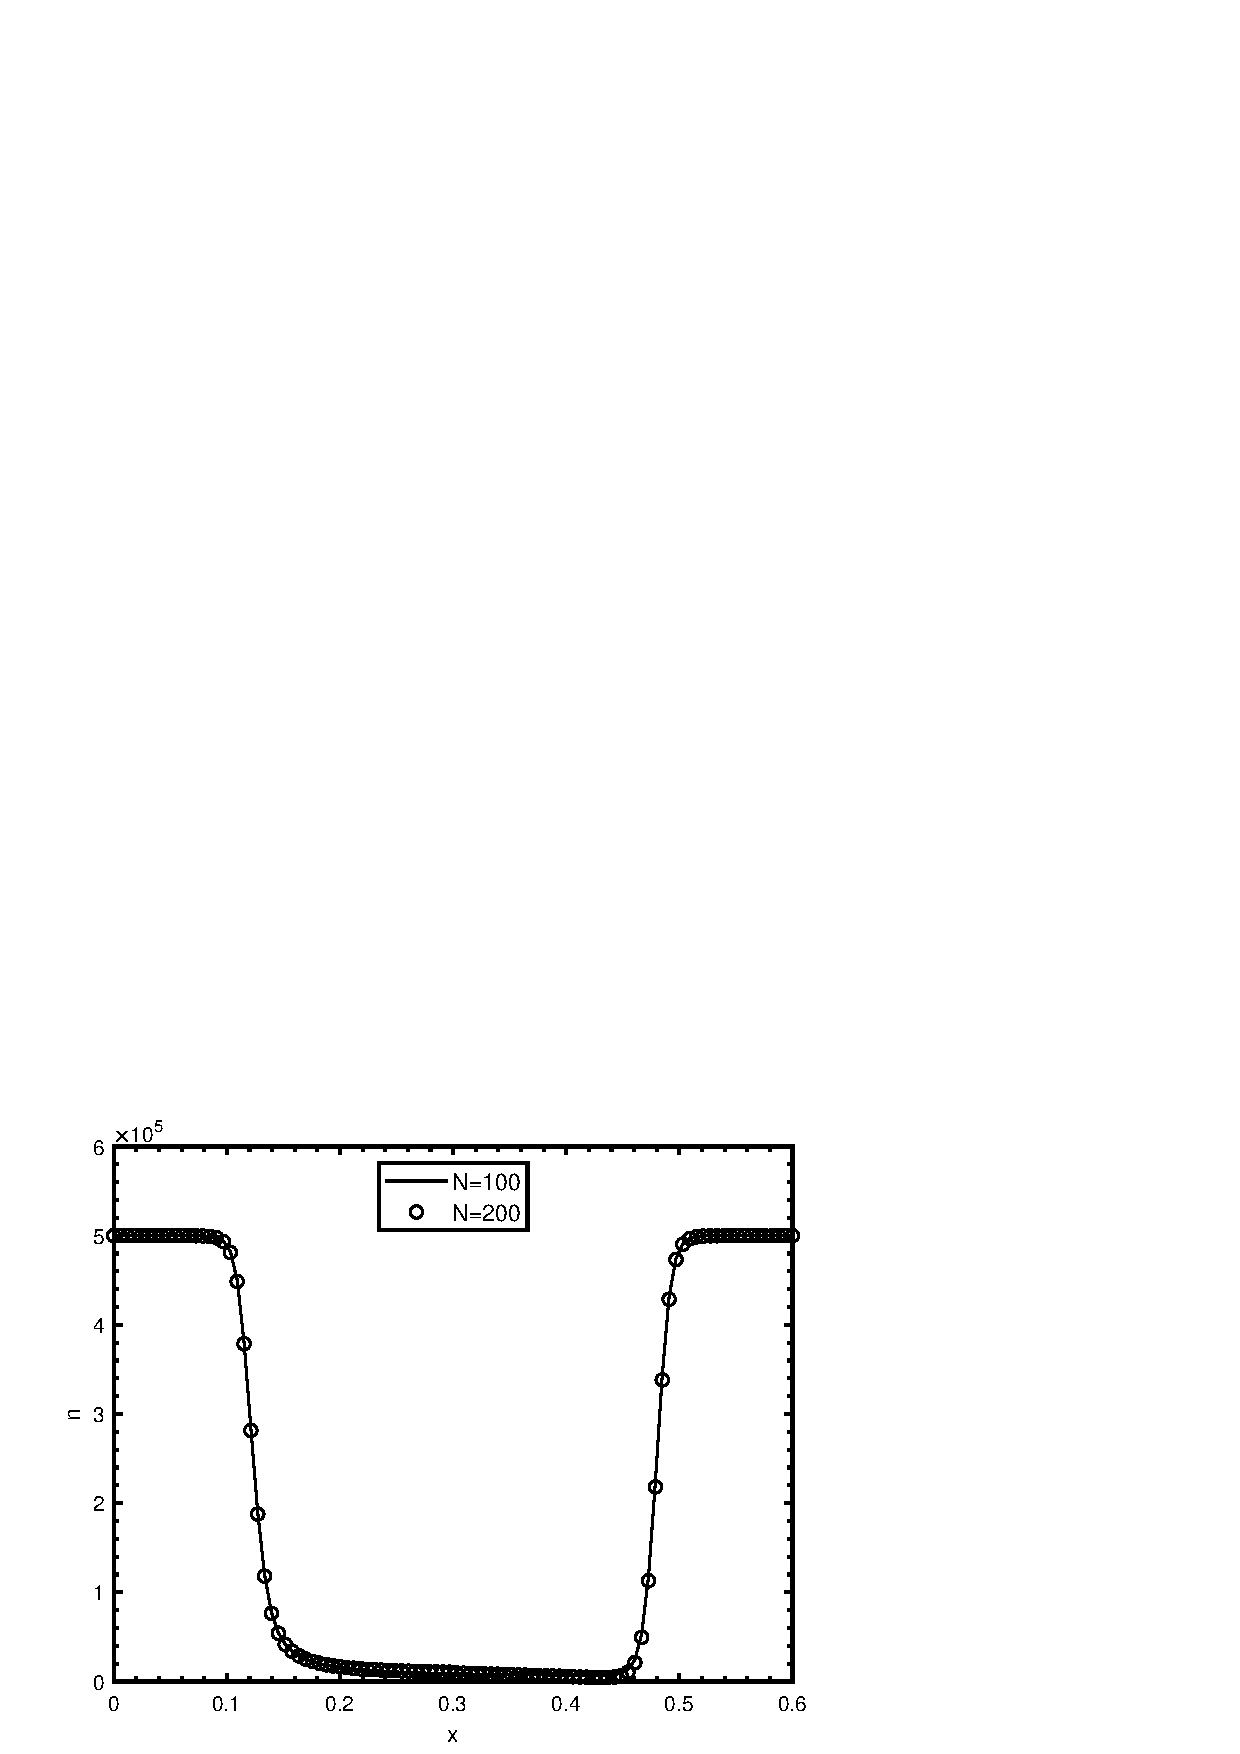
\includegraphics[width=\linewidth]{figure/DDTVDRK3Degree2mu0.75Nn.pdf}
    \end{minipage}
    \begin{minipage}[b]{0.48\textwidth}
        \centering
        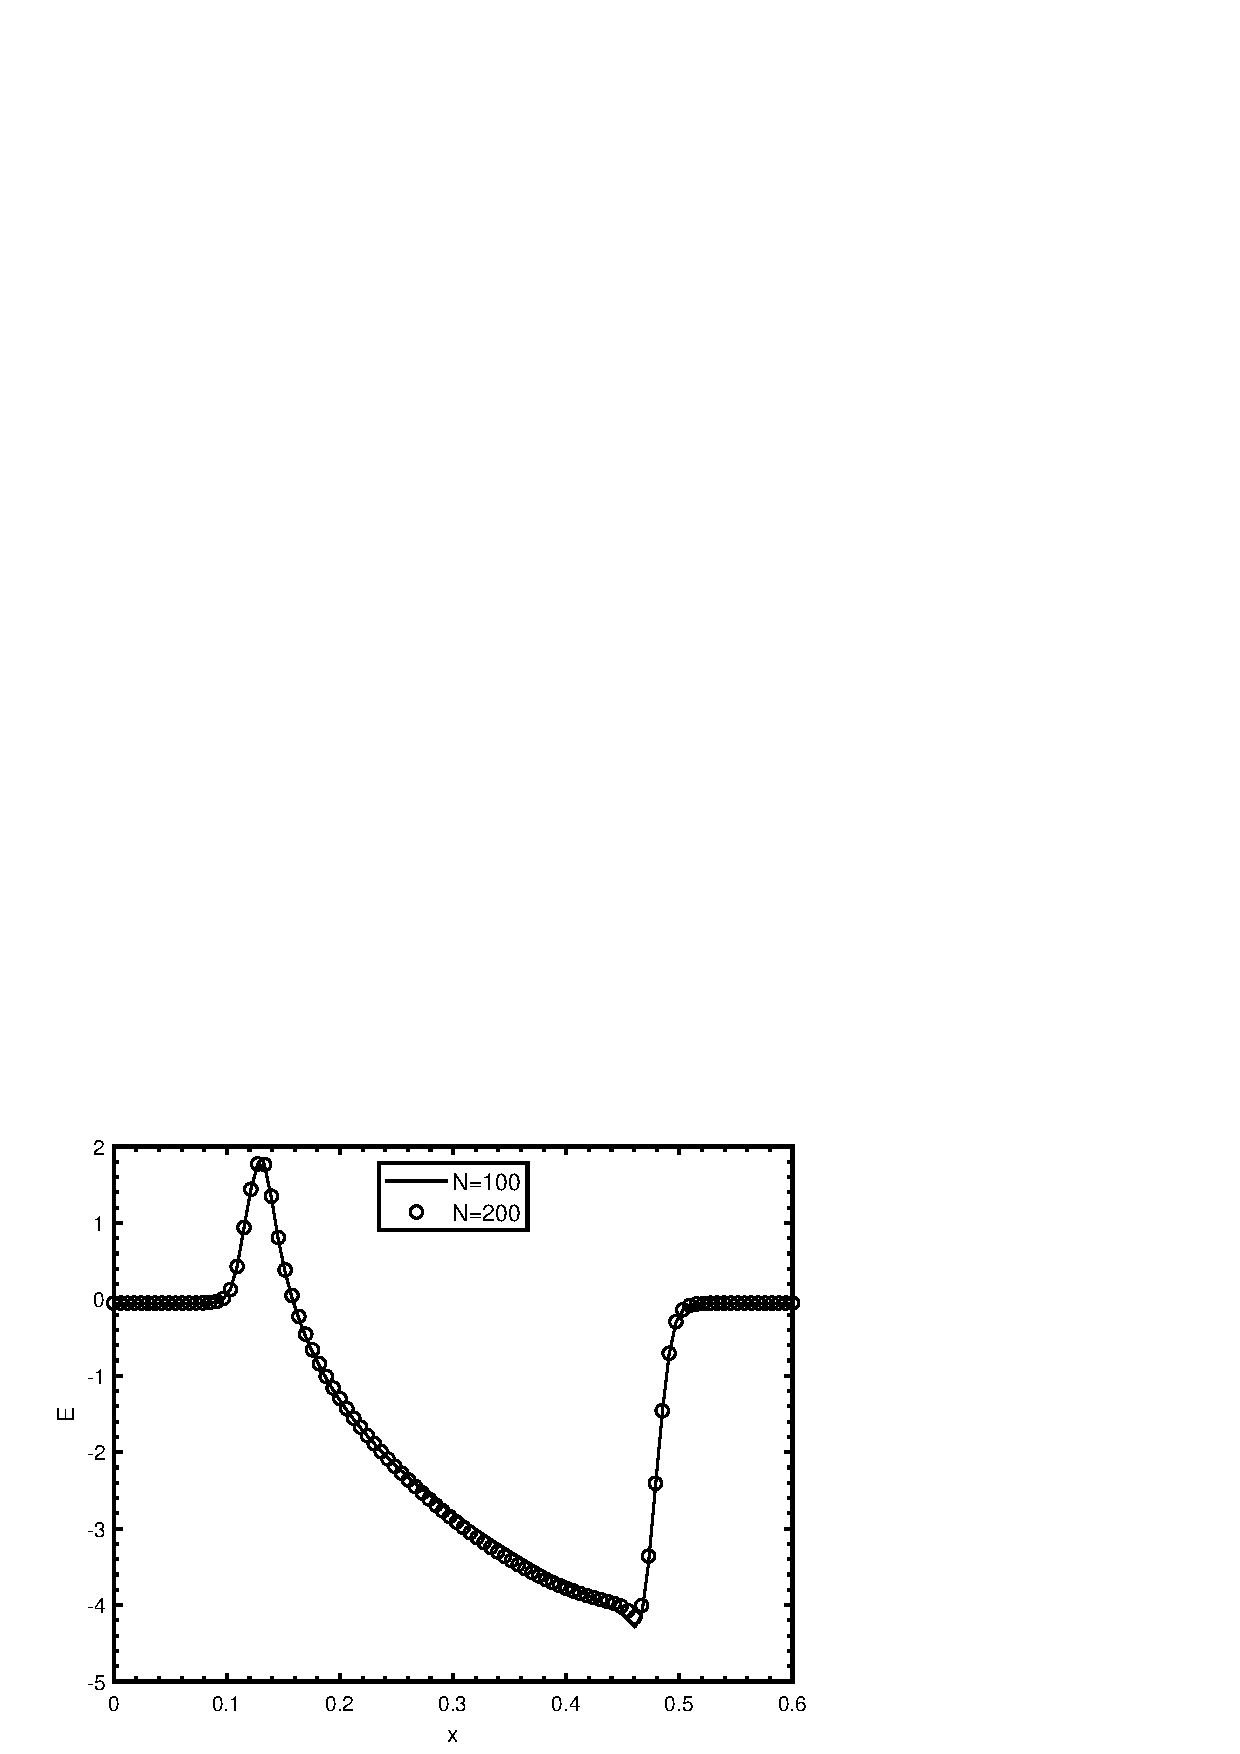
\includegraphics[width=\linewidth]{figure/DDTVDRK3Degree2mu0.75NE.pdf}
    \end{minipage}
    \caption{DD模型三阶TVDRK网格数N为100和200计算空间$V^2$。左:电子浓度n;右:电势E}
\end{figure}